\documentclass{report}\usepackage[]{graphicx}\usepackage[]{color}
%% maxwidth is the original width if it is less than linewidth
%% otherwise use linewidth (to make sure the graphics do not exceed the margin)
\makeatletter
\def\maxwidth{ %
  \ifdim\Gin@nat@width>\linewidth
    \linewidth
  \else
    \Gin@nat@width
  \fi
}
\makeatother

\definecolor{fgcolor}{rgb}{0.345, 0.345, 0.345}
\newcommand{\hlnum}[1]{\textcolor[rgb]{0.686,0.059,0.569}{#1}}%
\newcommand{\hlstr}[1]{\textcolor[rgb]{0.192,0.494,0.8}{#1}}%
\newcommand{\hlcom}[1]{\textcolor[rgb]{0.678,0.584,0.686}{\textit{#1}}}%
\newcommand{\hlopt}[1]{\textcolor[rgb]{0,0,0}{#1}}%
\newcommand{\hlstd}[1]{\textcolor[rgb]{0.345,0.345,0.345}{#1}}%
\newcommand{\hlkwa}[1]{\textcolor[rgb]{0.161,0.373,0.58}{\textbf{#1}}}%
\newcommand{\hlkwb}[1]{\textcolor[rgb]{0.69,0.353,0.396}{#1}}%
\newcommand{\hlkwc}[1]{\textcolor[rgb]{0.333,0.667,0.333}{#1}}%
\newcommand{\hlkwd}[1]{\textcolor[rgb]{0.737,0.353,0.396}{\textbf{#1}}}%

\usepackage{framed}
\makeatletter
\newenvironment{kframe}{%
 \def\at@end@of@kframe{}%
 \ifinner\ifhmode%
  \def\at@end@of@kframe{\end{minipage}}%
  \begin{minipage}{\columnwidth}%
 \fi\fi%
 \def\FrameCommand##1{\hskip\@totalleftmargin \hskip-\fboxsep
 \colorbox{shadecolor}{##1}\hskip-\fboxsep
     % There is no \\@totalrightmargin, so:
     \hskip-\linewidth \hskip-\@totalleftmargin \hskip\columnwidth}%
 \MakeFramed {\advance\hsize-\width
   \@totalleftmargin\z@ \linewidth\hsize
   \@setminipage}}%
 {\par\unskip\endMakeFramed%
 \at@end@of@kframe}
\makeatother

\definecolor{shadecolor}{rgb}{.97, .97, .97}
\definecolor{messagecolor}{rgb}{0, 0, 0}
\definecolor{warningcolor}{rgb}{1, 0, 1}
\definecolor{errorcolor}{rgb}{1, 0, 0}
\newenvironment{knitrout}{}{} % an empty environment to be redefined in TeX

\usepackage{alltt}
\IfFileExists{upquote.sty}{\usepackage{upquote}}{}
\begin{document}


Load timeCult file. Data are in raw condition.
\begin{knitrout}
\definecolor{shadecolor}{rgb}{0.969, 0.969, 0.969}\color{fgcolor}\begin{kframe}
\begin{alltt}
\hlcom{# setwd('C:/Dropbox/Workshop2013/Work/R/timeCult/') raw.data <-}
\hlcom{# read.csv('time2.csv',header=T,sep=',') head(raw.data) str(raw.data)}
\end{alltt}
\end{kframe}
\end{knitrout}


Select the rows you want to include in your analysis. Every row is a
tracked day.
\begin{knitrout}
\definecolor{shadecolor}{rgb}{0.969, 0.969, 0.969}\color{fgcolor}\begin{kframe}
\begin{alltt}
\hlcom{# hours <- raw.data[,c(1,3:4),drop=F] x <- hours[,] dim(x)}
\end{alltt}
\end{kframe}
\end{knitrout}


Save working data into a text file.\\
Remove header then replace ':' with '\t'.
\begin{knitrout}
\definecolor{shadecolor}{rgb}{0.969, 0.969, 0.969}\color{fgcolor}\begin{kframe}
\begin{alltt}
\hlcom{# write.table(x,'hours2.txt',sep='\textbackslash{}t',quote=F)}
\end{alltt}
\end{kframe}
\end{knitrout}


Read in the edited text file.\\
To convert hours into minutes, multiply V4 by 60.\\
Remove V6, the column that include the seconds.\\
Combine the sum V4 and V5 to unify the tracking of minutes.
\begin{knitrout}
\definecolor{shadecolor}{rgb}{0.969, 0.969, 0.969}\color{fgcolor}\begin{kframe}
\begin{alltt}
\hlstd{y} \hlkwb{<-} \hlkwd{read.table}\hlstd{(}\hlstr{"hours2.txt"}\hlstd{,} \hlkwc{sep} \hlstd{=} \hlstr{"\textbackslash{}t"}\hlstd{)}
\hlstd{y}\hlopt{$}\hlstd{V4} \hlkwb{<-} \hlstd{y}\hlopt{$}\hlstd{V4} \hlopt{*} \hlnum{60}
\hlstd{data.minutes} \hlkwb{<-} \hlkwd{data.frame}\hlstd{(}\hlkwc{day} \hlstd{= y}\hlopt{$}\hlstd{V2,} \hlkwc{subject} \hlstd{= y}\hlopt{$}\hlstd{V3,} \hlkwc{time} \hlstd{=} \hlkwd{rowSums}\hlstd{(y[,} \hlnum{4}\hlopt{:}\hlnum{5}\hlstd{]))}
\hlkwd{head}\hlstd{(data.minutes)}
\end{alltt}
\begin{verbatim}
##          day subject time
## 1 2013-03-16 Paper 3  180
## 2 2013-09-15 Paper 2  180
## 3 2013-09-16 Paper 1  259
## 4 2013-09-16    Idle   89
## 5 2013-09-16 Paper 1  178
## 6 2013-09-16    Idle   52
\end{verbatim}
\begin{alltt}
\hlstd{ordered.dat} \hlkwb{<-} \hlstd{data.minutes[}\hlkwd{order}\hlstd{(data.minutes[,} \hlnum{2}\hlstd{]), ]}
\hlkwd{head}\hlstd{(ordered.dat)}
\end{alltt}
\begin{verbatim}
##           day subject time
## 4  2013-09-16    Idle   89
## 6  2013-09-16    Idle   52
## 9  2013-09-17    Idle    0
## 10 2013-09-17    Idle  900
## 11 2013-09-17    Idle  159
## 13 2013-09-18    Idle    1
\end{verbatim}
\begin{alltt}
\hlkwd{summary}\hlstd{(ordered.dat)}
\end{alltt}
\begin{verbatim}
##          day            subject         time       
##  2013-11-29: 10   Idle      :300   Min.   :   0.0  
##  2013-09-24:  8   Paper 1   : 38   1st Qu.:   7.2  
##  2014-02-18:  8   Paper 2   : 70   Median : 103.5  
##  2013-09-21:  7   Paper 3   :111   Mean   : 184.9  
##  2013-10-05:  6   PostDoc   :  5   3rd Qu.: 307.5  
##  2014-01-31:  6   Soutenance:  7   Max.   :1633.0  
##  (Other)   :521   Thesis    : 35
\end{verbatim}
\end{kframe}
\end{knitrout}


Convert time back to hours.
Store data into a timeseries object.
Plot Paper 1
\begin{knitrout}
\definecolor{shadecolor}{rgb}{0.969, 0.969, 0.969}\color{fgcolor}\begin{kframe}
\begin{alltt}
\hlstd{ordered.dat}\hlopt{$}\hlstd{time} \hlkwb{<-} \hlstd{ordered.dat}\hlopt{$}\hlstd{time}\hlopt{/}\hlnum{24}
\hlstd{paper1} \hlkwb{<-} \hlstd{ordered.dat[ordered.dat[,} \hlnum{2}\hlstd{]} \hlopt \hlstr{"Paper 1"}\hlstd{, ]}
\hlkwd{summary}\hlstd{(paper1)}
\end{alltt}
\begin{verbatim}
##          day           subject        time       
##  2013-09-24: 4   Idle      : 0   Min.   : 0.583  
##  2013-09-16: 3   Paper 1   :38   1st Qu.: 4.000  
##  2013-09-21: 3   Paper 2   : 0   Median : 6.292  
##  2013-09-17: 2   Paper 3   : 0   Mean   : 7.012  
##  2013-09-18: 2   PostDoc   : 0   3rd Qu.: 9.542  
##  2013-09-20: 2   Soutenance: 0   Max.   :23.667  
##  (Other)   :22   Thesis    : 0
\end{verbatim}
\begin{alltt}
\hlstd{finaldat} \hlkwb{<-} \hlstd{paper1[}\hlkwd{order}\hlstd{(paper1[,} \hlnum{3}\hlstd{],} \hlkwc{decreasing} \hlstd{= T), ]}
\hlkwd{head}\hlstd{(finaldat)}
\end{alltt}
\begin{verbatim}
##           day subject  time
## 46 2013-09-25 Paper 1 23.67
## 50 2013-09-27 Paper 1 13.79
## 32 2013-09-22 Paper 1 13.67
## 20 2013-09-20 Paper 1 12.58
## 14 2013-09-18 Paper 1 12.21
## 36 2013-09-23 Paper 1 11.29
\end{verbatim}
\begin{alltt}
\hlstd{ts.min} \hlkwb{<-} \hlkwd{ts}\hlstd{(finaldat[}\hlopt{-}\hlnum{1}\hlstd{, ])}
\hlkwd{plot}\hlstd{(ts.min,} \hlkwc{plot.type} \hlstd{=} \hlstr{"single"}\hlstd{)}
\end{alltt}
\end{kframe}
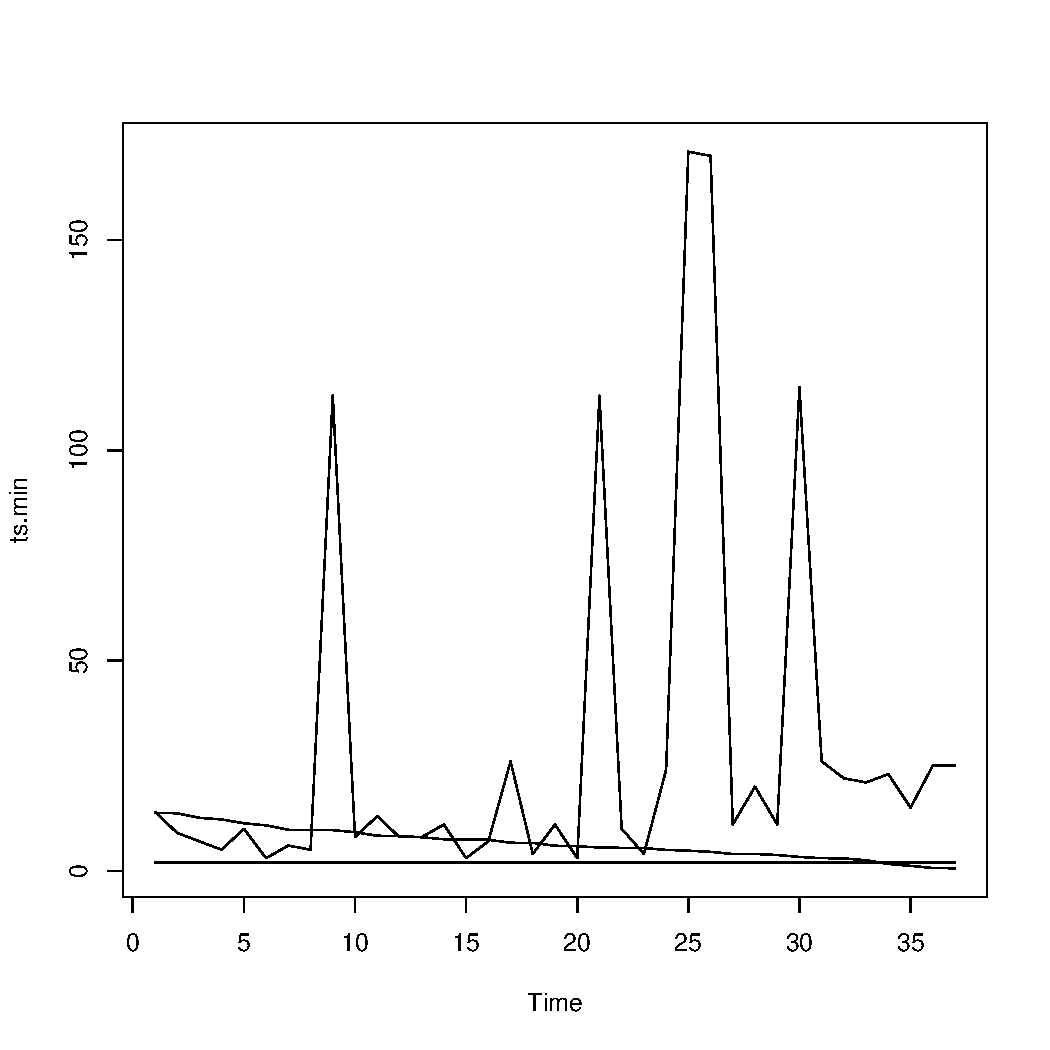
\includegraphics[width=\maxwidth]{figure/unnamed-chunk-5} 

\end{knitrout}



When working with dates
\begin{knitrout}
\definecolor{shadecolor}{rgb}{0.969, 0.969, 0.969}\color{fgcolor}\begin{kframe}
\begin{alltt}
\hlcom{# date <-strptime(as.character(date), '%m/%d/%y')}
\end{alltt}
\end{kframe}
\end{knitrout}


Plot using ggplot.
Scatterplot.
Although the idle time was removed for better interpretability.
\begin{knitrout}
\definecolor{shadecolor}{rgb}{0.969, 0.969, 0.969}\color{fgcolor}\begin{kframe}
\begin{alltt}
\hlstd{dat.less} \hlkwb{<-} \hlstd{ordered.dat[}\hlopt{!}\hlstd{ordered.dat}\hlopt{$}\hlstd{subject} \hlopt \hlstr{"Idle"}\hlstd{, ]}
\hlkwd{summary}\hlstd{(dat.less)}
\end{alltt}
\begin{verbatim}
##          day            subject         time      
##  2013-09-24:  4   Idle      :  0   Min.   : 0.00  
##  2014-02-18:  4   Paper 1   : 38   1st Qu.: 5.47  
##  2013-09-16:  3   Paper 2   : 70   Median :11.25  
##  2013-09-21:  3   Paper 3   :111   Mean   :11.75  
##  2013-10-05:  3   PostDoc   :  5   3rd Qu.:16.73  
##  2013-10-16:  3   Soutenance:  7   Max.   :29.00  
##  (Other)   :246   Thesis    : 35
\end{verbatim}
\begin{alltt}
\hlkwd{require}\hlstd{(ggplot2)}
\hlkwd{ggplot}\hlstd{(dat.less,} \hlkwd{aes}\hlstd{(day, time))} \hlopt{+} \hlkwd{geom_point}\hlstd{(}\hlkwd{aes}\hlstd{(}\hlkwc{size} \hlstd{= time,} \hlkwc{color} \hlstd{= subject))}
\end{alltt}
\end{kframe}
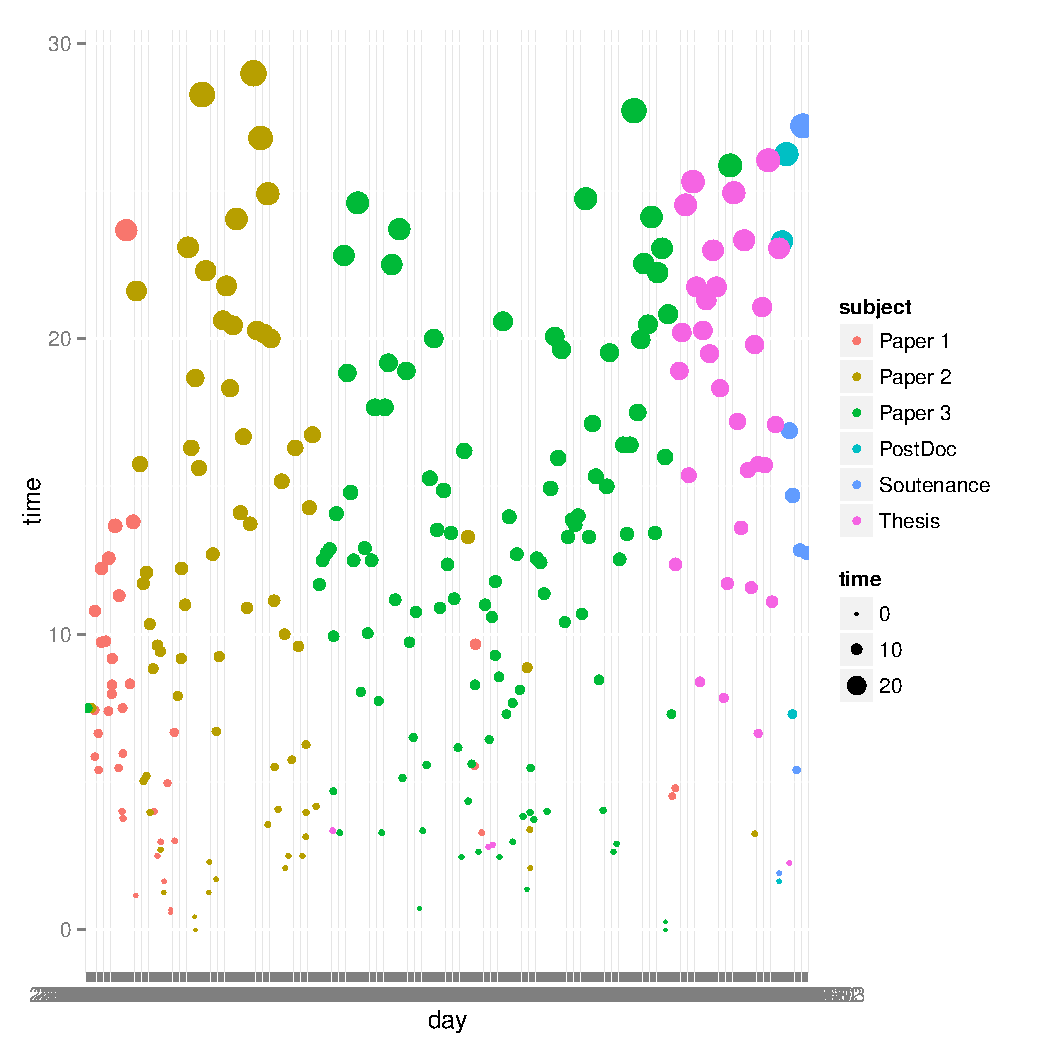
\includegraphics[width=\maxwidth]{figure/unnamed-chunk-7} 

\end{knitrout}



Barplot using ggplot but with the summary of all hours
\begin{knitrout}
\definecolor{shadecolor}{rgb}{0.969, 0.969, 0.969}\color{fgcolor}\begin{kframe}
\begin{alltt}
\hlstd{full.time} \hlkwb{<-} \hlkwd{read.table}\hlstd{(}\hlstr{"full.time.txt"}\hlstd{,} \hlkwc{sep} \hlstd{=} \hlstr{"\textbackslash{}t"}\hlstd{)}
\hlkwd{ggplot}\hlstd{(full.time,} \hlkwd{aes}\hlstd{(}\hlkwc{x} \hlstd{= V1,} \hlkwc{y} \hlstd{= V2))} \hlopt{+} \hlkwd{geom_bar}\hlstd{(}\hlkwc{colour} \hlstd{=} \hlstr{"black"}\hlstd{,} \hlkwc{fill} \hlstd{=} \hlstr{"#DD8888"}\hlstd{,}
    \hlkwc{width} \hlstd{=} \hlnum{0.7}\hlstd{,} \hlkwc{stat} \hlstd{=} \hlstr{"identity"}\hlstd{)}
\end{alltt}
\end{kframe}
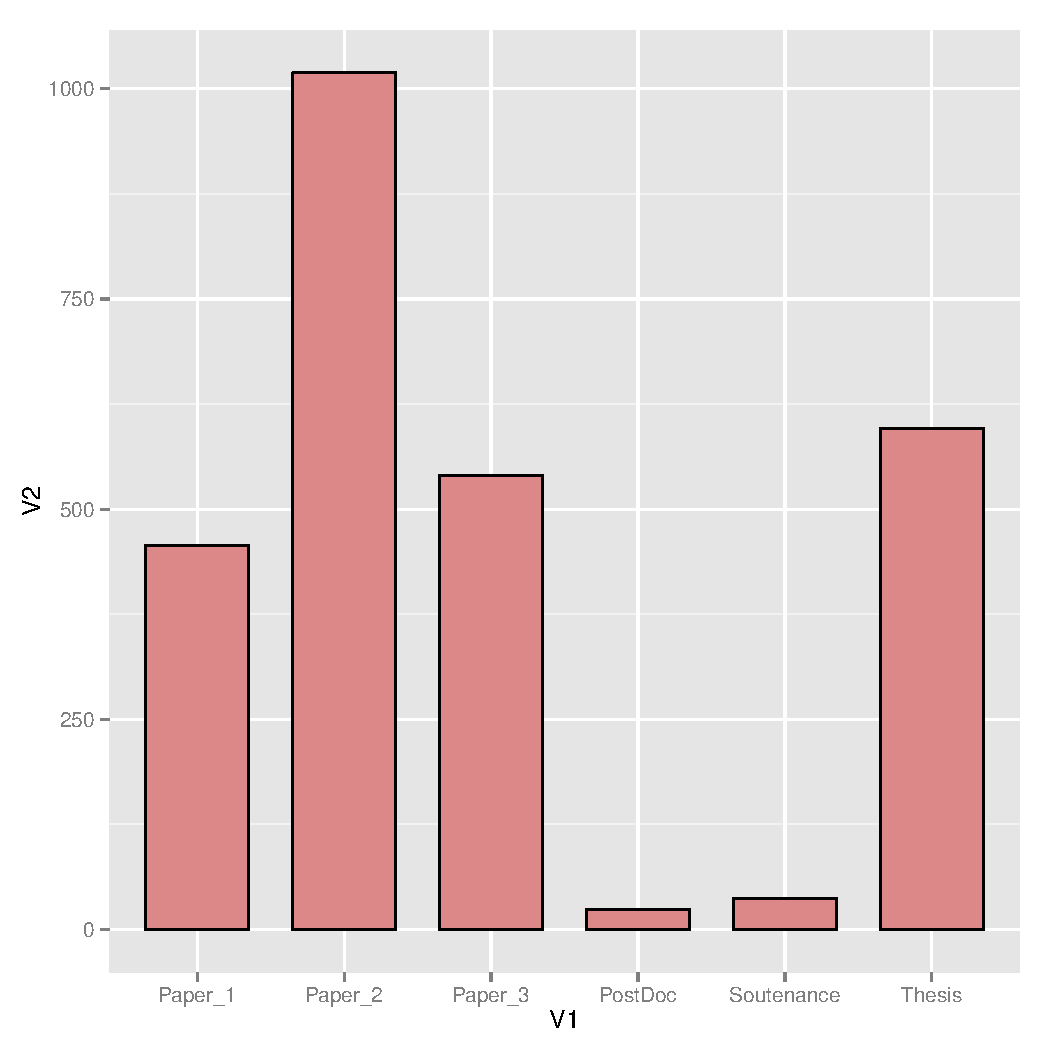
\includegraphics[width=\maxwidth]{figure/unnamed-chunk-8} 

\end{knitrout}








\end{document}


